%            PACKAGES AND OTHER DOCUMENT CONFIGURATIONS
%----------------------------------------------------------------------------------------
\documentclass[paper=letter,8.5pt]{article}
\usepackage[spanish]{babel} 
\decimalpoint
\usepackage{amsmath,amsfonts,amsthm} % Math packages
\usepackage{floatrow}
\usepackage{subfig}
\usepackage[utf8]{inputenc}
\usepackage{float}
\usepackage{lipsum} % Package to generate dummy text throughout this template
\usepackage{blindtext}
\usepackage{graphicx} 
\graphicspath{{Figuras/}} % Directory in which figures are stoorange
\usepackage[font=footnotesize,labelfont=bf]{caption}
\usepackage{subcaption}
%\usepackage{cmr} % Use the Palatino font
\usepackage{lmodern}
\usepackage[T1]{fontenc} % Use 8-bit encoding that has 256 glyphs
\linespread{1.05} % Line spacing - Palatino needs more space between lines
\usepackage{microtype} % Slightly tweak font spacing for aesthetics
\usepackage[hmarginratio=1:1,top=32mm,columnsep=20pt]{geometry} % Document margins
\usepackage{multicol} % Used for the two-column layout of the document
%\usepackage[hang, small,labelfont=bf,up,textfont=it,up]{caption} % Custom captions under/above floats in tables or figures
\usepackage[figurename=Fig.]{caption}
\usepackage{booktabs} % Horizontal rules in tables
\usepackage{float} % Required for tables and figures in the multi-column environment - they need to be placed in specific locations with the [H] (e.g. \begin{table}[H])
\usepackage{hyperref} % For hyperlinks in the PDF
\usepackage{wrapfig}
\usepackage{xcolor}
\usepackage{lettrine} % The lettrine is the first enlarged letter at the beginning of the text
\usepackage{paralist} % Used for the compactitem environment which makes bullet points with less space between them
\usepackage{abstract} % Allows abstract customization
\renewcommand{\abstractnamefont}{\normalfont\bfseries} % Set the "Abstract" text to bold
\renewcommand{\abstracttextfont}{\normalfont\small\itshape} % Set the abstract itself to small italic text
\usepackage{titlesec} % Allows customization of titles

\renewcommand\thesection{\Roman{section}} % Roman numerals for the sections
\renewcommand\thesubsection{\Roman{subsection}} % Roman numerals for subsections
\newcommand{\uvec}[1]{\hat{e}_{#1}}

\titleformat{\section}[block]{\large\scshape\centering}{\thesection.}{1em}{} % Change the look of the section titles
\titleformat{\subsection}[block]{\large}{\thesubsection.}{1em}{} % Change the look of the section titles
\newcommand{\horrule}[1]{\rule{\linewidth}{#1}} % Create horizontal rule command with 1 argument of height


%cambiar a negrita los numeros de las ecuaciones
%\makeatletter
%\def\tagform@#1{\maketag@@@{(\ignorespaces\textbf{#1}\unskip\@@italiccorr)}}
%\renewcommand{\eqref}[1]{\textup{{\normalfont(\ref{#1}}\normalfont)}}
%\makeatother

%---------------------------------------------------------------------------------------
%IMÁGENES INCLUIDAS


%----------------------------------------------------------------------------------
\hypersetup{colorlinks=true,linkcolor=blue,citecolor=blue,filecolor=blue,urlcolor=magenta,}

\usepackage{fancyhdr} % Headers and footers
\pagestyle{fancy} % All pages have headers and footers
\fancyhead{} % Blank out the default header
\fancyfoot{} % Blank out the default footer


\fancyhead[RO,LE]{Universidad Nacional Autónoma de México | Facultad de Ciencias | Servicio Social } % Custom header text
\renewcommand{\headrulewidth}{0.4pt}

\fancyfoot[RO,LE]{\thepage} % Custom footer text
\fancyheadoffset[RO,LE]{0.01\textwidth}


%----------------------------------------------------------------------------------------
%       TITLE SECTION
%----------------------------------------------------------------------------------------
\title{\vspace{-15mm}\fontsize{17pt}\selectfont\textbf{Cálculo de las secciones transversales de extinción, absorción y esparcimiento de elipsoides en la aproximación cuasiestática como primera aproximación de eritrocitos }} % Article title
\author{
\large
{\textsc{ Dana Larissa Luna González}}\\[2mm]}
\date{}
\geometry{total={170mm,230mm}, left=20mm, top=25mm}
 
\begin{document}
\maketitle % Insert title
\thispagestyle{fancy} % All pages have headers and footers
\floatsetup[figure]{style=plain,subcapbesideposition=top}
\section{Introducción}
El estudio de las propiedades ópticas de las células biológicas como los osteoblastos \cite{Osteoblastos}, los linfocitos \cite{Linfocitos}, y los eritrocitos \cite{Blood}, es de gran importancia para el área médica. A partir de las propiedades ópticas de las células, se obtiene información de su composición y estado morfológico, lo cual tiene potenciales aplicaciones en el diagnóstico y la detección temprana de diversas enfermedades, incluidos cánceres e infecciones virales \cite{Linfocitos}. En particular, el estudio de los eritrocitos tiene un papel importante en el diagnóstico de la anemia en sus diferentes tipos y el diseño de nuevas terapias ópticas, como el tratamiento de las venas varicosas \cite{Blood}. \\

Los eritrocitos sanos presentan forma de discoides cóncavos con longitudes de entre 4 a 9 mm de diámetro. Estos no poseen núcleo, por lo que pueden modelarse como un objeto homogéneo \cite{Cassini}. Debido a su forma, para simplificar el proceso de modelado, se han empleado diferentes opciones como los óvalos de Cassini \cite{Cassini} o funciones en términos de coordenadas esféricas \cite{Esferico}. Sin embargo, el modelo más simple a estudiar como una primera aproximación es un elipsoide. El objetivo este trabajo es el de analizar la convergencia y propiedades físicas de la respuesta óptica de elipsoides de diferentes materiales (oro, plata, aluminio, bismuto y óxido de magnesio) y tamaños dentro de la nanoescala, por medio de las secciones transversales de esparcimiento, absorción y extinción, bajo la aproximación cuasi-estática para, posteriormente, orientarlo a eritrocitos. En la primera sección de este trabajo, se resuelve de forma analítica el problema de esparcimiento de luz por una partícula elispoidal arbitraria en la aproximación cuasiestática, donde se presentan, además, la secciones tranversales de extinción, absorción y esparcimiento. Finalmente, se estudia el esparcimiento de luz por un elipsoide centrado en el origen en la aproximación cuasi-estática. En la segunda sección, se exponen los resultados obtenidos de las secciones transversales de extinción para partículas elipsoidales oblatas de materiales tanto plasmónicos como dieléctricos. En la última sección, denominada Resultados, se discute la implementación del método desarrollado para el caso de los eritrocitos.


\subsection{Aproximación cuasiestática en el problema de esparcimiento de luz por partículas elipsoidales}

 En el caso de un elipsoide caracterizado por una función dieléctrica $\epsilon_p$, que se encuentra inmerso en un medio caracterizado por una función dieléctrica $\epsilon_m$ y cuyo semieje mayor es $a$, se puede definir el límite cuasiestático cuando el parámetro de tamaño $x=ka$ es mucho menor que la unidad \cite{Bohren}, donde $k=2\pi \sqrt{\epsilon_m}/\lambda$ con $\lambda$ la longitud de onda. Esta aproximación garantiza que toda la geometría del elipsoide esté sujeta a un campo eléctrico de la misma intensidad y dirección \cite{Miguel}. En esta sección se estudiará el caso del dipolo eléctrico de una esfera para introducir el concepto de polarizabilidad, y más adelante, se desarrollará el dipolo eléctrico para esparcidores arbitrarios en donde se analizarán las regiones de campo cercano, la intermedia y la de radiación.


\subsubsection{Dipolo eléctrico (caso estático)}

En electrodinámica clásica, se entiende como \textit{límite cuasiestático} el considerar una partícula de tamaño mucho menor que la longitud de onda de la luz incidente \cite{Cuasiest}. Para el caso de una partícula esférica, se puede emplear la aproximación cuasiestática al resolver la ecuación de Laplace para el potencial eléctrico $\phi$. En particular, esta solución deviene en \cite{Griffiths}:
\begin{equation}
\phi=\frac{p}{4\pi\epsilon_m}\left(\frac{\Vec{r}\cdot\hat{e}_z}{r^3}\right)=\frac{\Vec{p}\cdot\Vec{r}}{4\pi\epsilon_m r^3}=\frac{p\cos\theta}{4\pi\epsilon_m r^2}
\label{pot_dipolo}
\end{equation}
donde $\Vec{p}$ representa el momento dipolar eléctrico. Si se considera una esfera con permitividad eléctrica $\epsilon_p$, embebida en el mismo medio caracterizado por su función dieléctrica $\epsilon_m$ en el cual existe un campo eléctrico uniforme $\Vec{E}_0=E_0\hat{e}_z$, al resolver la ecuación de Laplace considerando las condiciones de frontera entre la esfera y el medio, se obtiene que el campo eléctrico fuera de la esfera es la superposición del campo eléctrico aplicado y del campo eléctrico producido por un dipolo eléctrico puntual localizado en el origen con momento dipolar \cite{Bohren}:
\begin{equation}
	\vec{p}= \epsilon_m\alpha\Vec{E}_0=4\pi\epsilon_m a^3\frac{\epsilon_1-\epsilon_m}{\epsilon_1+2\epsilon_m}\Vec{E}_0, \;\text{con}\; \alpha=4\pi a^3(\epsilon_1-\epsilon_m)/(\epsilon_1+2\epsilon_m),
	\label{momentdipol}
\end{equation}
donde $\alpha$ es la polarizabilidad eléctrica, que representa la facilidad con la que se polariza la esfera. Es decir, el campo eléctrico induce un dipolo eléctrico en la esfera.
\begin{figure}[h!]
	\includegraphics[width=6cm]{../../Figuras/shereE0}
	\caption{Esfera de radio $r$ caracterizada por su función dieléctrica $\epsilon_p$ y embebida en un medio caracterizado por su función dieléctrica $\epsilon_$ en la cual incide un campo eléctrico uniforme $\Vec{E}_0$.}
\end{figure}


\subsubsection{Dipolo eléctrico (caso dinámico)}}

En la sección anterior se abordó una solución que asume que el campo eléctrico,  por tanto el dipolo inducido, son estáticos. Para resolver el caso dinámico en el límite cuasiestático, se asume ahora que las cargas están localizadas en un volumen finito moviéndose en presencia de un campo eléctrico dinámico; lo cual es equivalente a realizar un análisis en componentes de Fourier de los potenciales y campos de un sistema de cargas y corrientes localizadas en el espacio vacío, con una dependencia armónica $e^{-i\omega t}$, tal que varían en el tiempo y oscilan a la frecuencia $\omega$ del campo electromagnético aplicado. De esta forma, la densidad volumétrica de carga $\rho(\Vec{r},t)$ y la densidad de corriente $\Vec{J}(\Vec{r},t)$  en la posición $\Vec{r}$ se expresan como \cite{Jackson}
\begin{align}
    \rho(\Vec{r},t)&=\rho(\Vec{r})e^{-i\omega t},\nonumber\\
    \Vec{J}(\Vec{r},t)&=\Vec{J}(\Vec{r})e^{-i\omega t},
    \label{armonicf}
\end{align}
considerando que el significado físico lo posee la parte real. Mediante lo anterior, es posible determinar los campos electromagnéticos mediante el potencial vectorial como \cite{Jackson}:
\begin{align}
  \Vec{A}(\Vec{r},t)=\frac{\mu_0}{4\pi}\int \text{d}^3r'\frac{\Vec{J}(\Vec{r'})e^{i\omega \frac{|\Vec{r}-\Vec{r'}|}{c}}}{|\Vec{r}-\Vec{r'}|}e^{-i\omega t_r},
  \label{Achafa}
\end{align}
en donde se emplea la norma de Lorentz \cite{Griffiths} y la densidad de corriente se evalúa en el tiempo de retardo $t_r=t-|\Vec{r}-\Vec{r'}|/c$. \\

El comportamiento de los campos electromagnéticos se puede estudiar al delimitar diferentes regiones considerando valores extremos de $k=\omega/c$, como se verá a continuación. Empleando la definición anterior y obviando la dependencia temporal, la Ec. (\ref{Achafa}) se reescribe como
\begin{equation}
    \Vec{A}(\Vec{r},t)=\frac{\mu_0}{4\pi}\int \Vec{J}(\Vec{r'})\frac{e^{ik|\Vec{r}-\Vec{r'}|}}{|\Vec{r}-\Vec{r'}|} \text{d}^3r'.
    \label{pot_vectorial}
\end{equation} 
En la región de campo cercano, donde $r\ll\lambda$ (o $kr\ll 1$), tal que exp($ik|\Vec{r}-\Vec{r'}|)\to 1$, se tiene \cite{Jackson}
\begin{equation*}
	\Vec{A}(\Vec{r},t)=\frac{\mu_0}{4\pi}\int \frac{\Vec{J}(\Vec{r'})}{|\Vec{r}-\Vec{r'}|} \text{d}^3r',
\end{equation*} 
mientras que en la región de campo lejano ($kr\gg 1$) dado que la exponencial oscila rápidamente, es suficiente aproximar
\begin{equation}
	|\Vec{r}-\Vec{r'}|\simeq r-\hat{e}_r\cdot\Vec{r'},    
\end{equation}
con $\hat{e}_r$ un vector unitario en la dirección de $\Vec{r}$. \footnote{Empleando la ley de cosenos y haciendo una expansión binomial $
	|\Vec{r}-\Vec{r'}|=\sqrt{r^2+(r')^2-2rr'\cos\theta}=r\sqrt{1+\left(r'/r\right)^2-2\left((r'/r)\cos\theta\right)}\simeq r\left\{1-(\hat{e}_r\cdot\Vec{r'}/r)+1/2\left(r'/r\right)^2\right\}\simeq r-\hat{e}_r\cdot\Vec{r'}.$} 	
	Si sólo se consideran los términos que decaen como $r^{-1}$, el inverso de la distancia en la Ec. (\ref{pot_vectorial}) puede ser reemplazado por $r$. Entonces, el potencial vectorial es
	\begin{equation*}
	\lim_{kr\rightarrow\infty}\Vec{A}(\Vec{r})=\frac{\mu_0}{4\pi}\frac{e^{ikr}}{r}\int \Vec{J}(\Vec{r'})e^{-ik\hat{e}_r\cdot\Vec{r'}}\text{d}^3r',    
	\end{equation*}
	que se puede reescribir al realizar la expansión en serie de potencias de la exponencial dentro de la integral de volumen, dando como resultado
	\begin{equation*}
	\lim_{kr\rightarrow\infty}\Vec{A}(\Vec{r})=\frac{\mu_0}{4\pi}\frac{e^{ikr}}{r}\sum_n\frac{(-ik)^n}{n!}\int \Vec{J}(\Vec{r'})(\hat{e}_r\cdot\Vec{r'})^n \text{d}^3r'.    
	\end{equation*}
\begin{figure}[h!]
	\includegraphics[width=6cm]{../../Figuras/aprox.jpg}
	\caption{Vector de posición $\Vec{r}$ del volumen y $\Vec{r'}$. Se muestra la distancia $|\Vec{r}-\Vec{r'}|$ entre estos últimos. }
\end{figure}
Al considerar únicamente el primer término de la expansión, se concluye que 
\begin{equation}
    \Vec{A}(\Vec{r})\approx\frac{\mu_0}{4\pi}\frac{e^{ikr}}{r}\int \Vec{J}(\Vec{r'}) \text{d}^3r',    
    \label{aprox_pot_vec}
\end{equation}
que al realizar una integración por partes,  \footnote{Al considerar $\int_V \Vec{r'}(\nabla'\cdot\Vec{J})\text{d}^3r'=\int_{\partial V} \Vec{r'}(\Vec{J}\cdot \text{d}\Vec{S})-\int_V \Vec{J}\text{d}^3r'$ y asumiendo que $\Vec{J}$ se desvanece en los límites del volumen $V$, es decir, en la superficie $\partial V$. } se obtiene que
\begin{equation}
	\int\Vec{J}d^3r'=-\int \Vec{r'}(\nabla'\cdot\Vec{J})\text{d}^3r'=-i\omega\int \Vec{r'}\rho(\Vec{r'})\text{d}^3r',
	\label{Jrho}
\end{equation}
donde se emplea la ecuación de continuidad
\begin{equation*}
    \nabla\cdot\Vec{J}=-\frac{\partial\rho}{\partial t}=i\omega\rho(\Vec{r}). 
\end{equation*}
Al sustituir la Ec. (\ref{Jrho}) en la Ec. (\ref{aprox_pot_vec}) y considerando que el momento dipolar eléctrico $\Vec{p}$ de una distribución de cargas $\rho$ es
\begin{equation*}
	\Vec{p}=\int \Vec{r'}\rho(\Vec{r'})\text{d}^3r',
\end{equation*}
se obtiene 
\begin{equation}
    \Vec{A}(\Vec{r})=-\frac{i\omega\mu_0}{4\pi}\frac{e^{ikr}}{r}\int \Vec{r'}\rho(\Vec{r'})\text{d}^3r'=-\frac{i\omega\mu_0}{4\pi}\frac{e^{ikr}}{r}\Vec{p}. 
    \label{A_dip}  
\end{equation}
Al calcular el campo $\Vec{H}$ como función del potencial vectorial, y empleando la ley de Faraday-Lenz para determinar el campo eléctrico, se concluye que \cite{Jackson}
\begin{align}
	\Vec{E}&=\frac{1}{4\pi\epsilon_0}\left\{k^2(\hat{e}_r\times\Vec{p})\times\hat{e}_r\frac{e^{ikr}}{r}+[3\hat{e}_r(\hat{e}_r\cdot\Vec{p})-\Vec{p}]\left(\frac{1}{r^3}-\frac{ik}{r^2}\right)e^{ikr}\right\},\label{E}\\
    \Vec{H}&=\frac{ck^2}{4\pi}(\hat{e}_r\times\Vec{p})\frac{e^{ikr}}{r}\left(1-\frac{1}{ikr}\right).    \label{H}
\end{align}
A partir de las Ecs. (\ref{E})  y (\ref{H}) se puede observar que el campo $\Vec{H}$ es transversal al vector radial para cualquier distancia, mientras el campo eléctrico tiene componentes paralelas y perpendiculares a $\hat{e}_r$.\\ 

 De forma análoga al desarrollo de la Ec. (\ref{A_dip}) y empleando la Ley de Faraday Lenz, en la zona de radiación cuando $kr\gg 1$, se tiene que al excitar a las fuentes en el sistema mediante una onda electromagnética de frecuencia angular $\omega$, lo que sería equivalente a iluminar al sistema con una onda plana armónica en el tiempo, se induce un dipolo eléctrico $\Vec{p}$ que genera campos electromagnéticos $\Vec{E}_p$ y $\Vec{H}_p$ y  que oscilan a la misma frecuencia $\omega$ 
\begin{align}
    \Vec{E}_p&=\frac{e^{ikr}}{-ikr}\frac{ik^3}{4\pi\epsilon_m}\hat{e}_r\times(\hat{e}_r\times \Vec{p}) e^{i\omega t}, \hspace{1cm}
    \Vec{H}_p=\frac{ck^2}{4\pi}(\hat{e}_r\times\Vec{p})\frac{e^{ikr}}{r}e^{i\omega t}.
\end{align}
En el caso particular en que el sistema se ilumine con una onda plana monocromática, es decir, de una sola frecuencia, y polarizada en la dirección $\hat{e}_x$, que induce un dipolo eléctrico con momento dipolar  $\Vec{p}=\epsilon_m \alpha E_0 e^{-i\omega t}\hat{e}_x$, se pueden reescribir a los campos generados por el dipolo inducido mediante el vector de amplitud de esparcimiento
\begin{equation}
	\Vec{X}=\frac{ik^3}{4\pi}\alpha \left( \hat{e}_r\times(\hat{e}_r\times \hat{e}_x)\right),
	\label{Xvec}
\end{equation}
como
 \begin{align}
 	\Vec{E}_{p}&=\frac{e^{ik(r-z)}}{-ikr}\Vec{X}\:E_0 e^{ikz},
 	\hspace{1cm}
 	\Vec{H}_{p}=\frac{k}{\omega\mu}\hat{e}_r\times\Vec{E}_{p}.
 	\label{EH_s}
 \end{align}
donde la polarización en la base de vectores esféricos es $\Vec{p}=\epsilon_m \alpha E_0 e^{-i\omega t}(\sin\theta\cos\phi\: \hat{e}_r+\cos\theta\cos\phi\: \hat{e}_{\theta}-\sin\phi \:\hat{e}_{\phi})$. \footnote{Es decir, $\hat{e}_r\times(\hat{e}_r\times \hat{e}_x)=-\cos\theta\cos\phi \hat{e}_{\theta}+\sin\phi \hat{e}_{\phi}$. } \\


\subsection{Secciones transversales}
Si se considera una partícula embebida en un medio no absorbente iluminada por una onda plana\footnote{Se puede generalizar a campos electromagnéticos arbitrarios al reconstruir dicho campo ondas planas debido al teorema de Fourier} y se construye una esfera imaginaria de radio $r$ alrededor de esta [Fig. \ref{WA}],  la energía electromagnética por unidad de tiempo que cruza la superficie $A$ de la esfera es
\begin{equation*}
	W_a=-\int_A \Vec{S}\cdot\hat{e}_rdA \footnote{Esta expresión se puede considerar como una medida de la cantidad de líneas de campo que atraviesan la superficie de integración, cuando $W_{a}>0$ entran más líneas de campo a la superficie cerrada en comparación con las que salen, por lo que se puede concluir que hay algún proceso por el cual se atenúa el campo electromagnético en el interior de la superficie. Mientras que cuando $W_{a}<0$, salen más líneas de campo hacia la superficie con respecto a la cantidad de líneas que entran en la misma. Este último caso no es considerado en el análisis pues implicaría que la energía se está creando en el interior de la partícula.},
	\label{flujopoynting}
\end{equation*}

donde $\Vec{S}=\Vec{E}\times\Vec{H}$ es el vector de Poynting. Dado que el vector de Poynting en cualquier punto en el medio que rodea a la partícula se puede considerar como la suma de los términos $\Vec{S}_i, \Vec{S}_s$ y $\Vec{S}_{ext}$  \cite{Bohren} asociados al campo incidente, al campo esparcido y a la interacción entre los dos anteriores\footnote{$\Vec{S}_{ext}=1/2\:\mbox{Re}\{\Vec{E}_i\times\Vec{H}_s^*+\Vec{E}_s\times\Vec{H}_i^*\}$ }, respectivamente, se tendrá que $W_a=W_i-W_s+W_{ext}$, donde
\begin{subequations}
	\begin{align}
			W_i & = -\int_{A}\Vec{S}_i\cdot\hat{e}_rdA 
		&& (\stepcounter{equation}\hypertarget{eq:Hom1}{\text{\theequation}}) 
		& W_s &=\int_{A}\Vec{S}_s\cdot\hat{e}_rdA \label{eq:MW1a}&& (\stepcounter{equation}\hypertarget{eq:Hom1}{\text{\theequation}}) &
		W_{ext}& = -\int_{A}\Vec{S}_{ext}\cdot\hat{e}_rdA. && (\stepcounter{equation}\hypertarget{eq:Hom2}{\text{\theequation}}) & \nonumber
	\end{align}
\end{subequations}
Para un medio no absorbente, $W_i$ es igual en todas partes, por lo que se anula\footnote{$W_i =\int_{0}^{\pi}\int_{0}^{2\pi}|S_i(r,\theta,\phi)|\cos\theta \sin\theta \: d\theta=0$}, entonces
\begin{equation}
	W_{ext}=W_a+W_s.
\end{equation}
\begin{figure}[h!]
	\centering
	\includegraphics[width=6cm]{../../Figuras/WA}
	\caption{Esquema de la esfera imaginaria  de radio $r$ y superficie $A$ centrada en el origen y en la partícula de interés.}
	\label{WA}
\end{figure}

Si se considera el campo incidente $\Vec{E_i}=E\hat{e}_x$ polarizado en la dirección $\hat{e}_x$ y a $\Vec{H}_i=(1/\mu \omega)\: \Vec{k} \times E \hat{e}_x$ en un medio no absorbente, $W_a$ es independiente del radio $r$ de la esfera imaginaria, por lo que se puede considerar al radio lo suficientemente grande para estar en la región de campo lejano donde los campos se comportan como las Ecs. (\ref{E_scat}) y (\ref{H_scat}), por lo cual, $W_{ext}$ estará dado por \cite{Bohren}
\begin{equation*}
	W_{ext}=I_i\frac{4\pi}{k^2}\:\text{Re}\{(\Vec{X}\cdot\hat{e}_x)_{\theta=0}\},
\end{equation*}
donde $I_i$ es la irradiancia incidente y por consiguiente,
\begin{equation}
	C_{ext}=\frac{W_{ext}}{I_i}=\frac{4\pi}{k^2}\:\text{Re}\{(\Vec{X}\cdot\hat{e}_x)_{\theta=0}\},\label{C_ext}
\end{equation}
que es la sección de área transversal de extinción y que posee dimensiones de área. La Ec.(\ref{C_ext}) puede ser rescrita como
\begin{equation}
	C_{ext}=C_{abs}+C_{sca}
\end{equation}
donde $C_{abs}=W_{abs}/I_i$ y $C_{sca}=W_s/I_i$ corresponden a las secciones transversales de absorción y esparcimiento, respectivamente. Al sustituir las Ecs. (\ref{E_scat}) y (\ref{H_scat}) en la Ec.(\hyperlink{23b}{}) se obtiene
\begin{equation}
	C_{sca}=\int_0^{2\pi}\int_0^{\pi}\frac{|\Vec{X}|^2}{k^2}\:\sin\theta\: d\theta\:d\phi.
	\label{C_sca}
\end{equation}
Estos coeficientes son propiedades macroscópicas y medibles, que proveen información sobre la energía absorbida y esparcida por un partícula. Debido al teorema óptico, la extinción solo depende del esparcimiento en la dirección de propagación y es el efecto combinado de la absorción en la partícula y el esparcimiento por la partícula en todas las direcciones. \\

\noindent Considerando al vector de amplitud de esparcimiento 
\begin{equation*}
	\Vec{X}\cdot\hat{e}_x=\frac{ik^3}{4\pi}\alpha \hat{e}_r\times(\hat{e}_r\times \hat{e}_x)\cdot\hat{e}_x=\frac{ik^3}{4\pi}\alpha\left(\hat{e}_r(\hat{e}_r\cdot \hat{e}_x)-\hat{e}_x(\hat{e}_r\cdot \hat{e}_r)\right)\cdot\hat{e}_x=\frac{ik^3}{4\pi}\alpha(\sin^2\theta\cos^2\phi-1),  
\end{equation*}
y sustituyéndolo en la Ec.(\ref{C_ext}), la sección transversal de extinción es
\begin{equation*}
	C_{ext}=k \mbox{Re}\left[\left(i\alpha(\sin^2\theta\cos^2\phi-1)\right)_{\theta=0}\right]=k\:\mbox{Re}\left[-i\alpha\right],
\end{equation*}
pero la polarizabilidad es compleja $\alpha=\alpha_1+i\alpha_2$, por lo que $-i\alpha=\alpha_2-i\alpha_1$; de forma que la parte real de $-i\alpha$ es igual a la parte imaginaria de $\alpha$, por lo que se sigue que
\begin{equation}
	C_{ext}=k\: \mbox{Im}[\alpha].    
\end{equation}
Asimismo, a partir de la Ec.(\ref{C_sca}) la sección transversal de esparcimiento se describe por
\begin{align}
	C_{sca}&=\int_{0}^{2\pi}\int_0^{\pi}\frac{|\Vec{X}|^2}{k^2}\sin\theta d\theta d\phi\nonumber\\
	&=\frac{(\alpha\cdot\alpha^*)k^4}{(4\pi)^2}\int_0^{2\pi}\int_0^{\pi}(\sin^2\theta\cos^2\phi+1)\sin\theta d\theta d\phi\nonumber\\
	&=\frac{|\alpha|^2k^4}{(4\pi)^2}\frac{8\pi^2}{3}=\frac{|\alpha|^2k^4}{6\pi}.
\end{align}
\subsection{Elipsoide en la aproximación cuasiestática}
En esta sección se busca estudiar el esparcimiento de luz por un elipsoide centrado en el origen, con semiejes ($a,b,c$) paralelos a los ejes $\uvec{x},\uvec{y},\uvec{z}$ respectivamente, y con dimensiones tales que $\lambda\gg a>b>c$. Mediante las cordenadas elipsoidales confocales \footnote{Existen diversas definiciones que pueden revisarse en \cite{Math}, sin embargo, se emplea la proporcionada en \cite{Arfken}. } [ver Fig. \ref{elipse}] se puede obtener una solución analítica (pero aproximada) al problema de esparcimiento de luz por un elipsoide. Estas describen la superficie del elipsoide como \cite{Math}
\begin{equation}
	\frac{x^2}{a^2-u}+\frac{y^2}{b^2-u}+\frac{z^2}{c^2-u}=1,
	\label{elipsoide2}
\end{equation}
 donde debe determinarse el valor del parámetro $u$. La Ec. (\ref{elipsoide2}) es una ecuación de tercer grado para $u$, por lo que las soluciones (reales) son un conjunto de tres valores $\{\xi,\eta,\zeta\}$ tales que \footnote{La función $f(u)=x^2/(a^2-u)+y^2/(b^2-u)+z^2/(c^2-u)-1$ resulta ser continuamente diferenciable en el dominio $(-\infty, c^2)\cap (c^2, b^2)\cap (b^2, a^2)$ y estrictamente creciente en cada intervalo que lo compone, de tal forma que, al calcular los límites en cada extremo de los intervalos, se concluye que existe exactamente una raíz en cada intervalo.}
\begin{equation}
	-\infty<\xi<c^2<\eta<b^2<\zeta<a^2
\end{equation}
que corresponden a tres formas cuadráticas con focos en común.
\begin{align}
    \frac{x^2}{a^2-\xi}+\frac{y^2}{b^2-\xi}+\frac{z^2}{c^2-\xi}=1,\\
    \frac{x^2}{a^2-\eta}+\frac{y^2}{b^2-\eta}+\frac{z^2}{c^2-\eta}=1,\\
    \frac{x^2}{a^2-\zeta}+\frac{y^2}{b^2-\zeta}+\frac{z^2}{c^2-\zeta}=1.
\end{align}
Si $\xi$ es constante, se obtiene un elipsoide confocal. De esta forma, la superficie de la partícula a estudiar se tiene cuando $\xi=0$. Cuando $\eta$ es constante, se obtiene un hiperboloide de una hoja y cuando $\zeta$ es constante se tiene un hiperboloide de dos hojas.\\

\noindent Es así como, a cualquier punto ($x,y,z$) le corresponde un conjunto de coordenadas elipsoidales ($\xi,\eta,\zeta$). Sin embargo, esto no es cierto para el caso contrario. Estas coordenadas determinan ocho puntos simétricamente localizados en los octantes cuyo espacio está particionado por los ejes coordenados $x,y,z$ anteriormente mencionados.\\
\begin{figure}[H]
    \centering
    \includegraphics[width=8cm]{../../Figuras/ellipsoid.png}    
    \caption{Sistema coordenado elipsoidal con un elipsoide centrado en el origen, con semiejes ($a, b, c$), $a > b > c.$}
    \label{elipse}
\end{figure}
\noindent Las ecuaciones anteriores se pueden reescribir de forma matricial como
\begin{center}
	\resizebox{0.44\textwidth}{!}{
		\begin{equation*}
			\begin{pmatrix}
				\frac{1}{a^2+\xi} & \frac{1}{b^2+\xi} & \frac{1}{c^2+\xi}\\
				\frac{1}{a^2+\eta} & \frac{1}{a^2+\eta} & \frac{1}{a^2+\eta}\\
				\frac{1}{a^2+\zeta} & \frac{1}{a^2+\zeta} & \frac{1}{a^2+\zeta}\end{pmatrix}\begin{pmatrix}
				x^2\\
				y^2\\
				z^2
			\end{pmatrix}=\begin{pmatrix}
				1\\
				1\\
				1\\
			\end{pmatrix},
		\end{equation*}
	}
\end{center}
cuya solución está dada por las expresiones
\begin{align}
    x^2&=\frac{(a^2+\xi)(a^2+\eta)(a^2+\zeta)}{(b^2-a^2)(c^2-a^2)},\label{x_elips}\\
     y^2&=\frac{(b^2+\xi)(b^2+\eta)(b^2+\zeta)}{(a^2-b^2)(c^2-b^2)},\label{y_elips}\\
     z^2&=\frac{(c^2+\xi)(c^2+\eta)(c^2+\zeta)}{(a^2-c^2)(b^2-c^2)}. \label{z_elips}    
\end{align}

En el problema de esparcimento de luz sin retardo (o límite cuasiestático) se resuelve la ecuación de Laplace para el potencial eléctrico; en un sistema coordenado general, esta ecuación se escribe en términos de coordenadas generalizadas \cite{Arfken}
\begin{equation}
	\nabla^2\phi=\frac{1}{h_1h_2h_3}\left[\frac{\partial}{\partial q_1}\left(\frac{h_2h_3}{h_1}\frac{\partial\phi}{\partial q_1}\right)+\frac{\partial}{\partial q_2}\left(\frac{h_3h_1}{h_2}\frac{\partial\phi}{\partial q_2}\right)+\frac{\partial}{\partial q_3}\left(\frac{h_1h_2}{h_3}\frac{\partial\phi}{\partial q_3}\right)\right],
	\label{laplaciano}    
\end{equation}
donde $\phi$ es una función escalar, y  $h_i$ con $i=1,2,3$ los factores de escala que, para coordenadas elipsoidales se asocian como $1\rightarrow\xi, 2\rightarrow\eta$ y $3\rightarrow\zeta,$ y se determinan al hacer un cambio de base de coordenadas cartesianas a elipsoidales. Para ello, se encuentra un vector unitario en la dirección de la i-ésima coordenada, que mide cómo es que cambia el vector posición $\vec{r}=(x,y,z)$ en una dirección dada y se define como \cite{Arfken}
\begin{equation}
	\uvec{i}=\frac{1}{h_i}\left(\frac{\partial \Vec{r}}{\partial q_i}\right),     
\end{equation}
con
\begin{equation}
	h_i=\Big|\frac{\partial \Vec{r}}{\partial q_i}\Big|=\sqrt{\left(\frac{\partial x}{\partial q_i}\right)^2+\left(\frac{\partial y}{\partial q_i}\right)^2+\left(\frac{\partial z}{\partial q_i}\right)^2}.
\end{equation} 
En particular, para el caso de coordenadas elipsoidales, considerando la variación en la dirección $x$, empleando la Ec. (\ref{x_elips}), se tiene que \begin{align*}
	\frac{\partial x}{\partial \xi}&=\frac{1}{2}\left(\frac{(a^2+\xi)(a^2+\eta)(a^2+\zeta)}{(b^2-a^2)(c^2-a^2)}\right)^{-1/2}\frac{\partial}{\partial \xi}\left(\frac{(a^2+\xi)(a^2+\eta)(a^2+\zeta)}{(b^2-a^2)(c^2-a^2)}\right)\nonumber\\
	&=\frac{1}{2}\frac{1}{a^2+\xi}\sqrt{\frac{(a^2+\xi)(a^2+\eta)(a^2+\zeta)}{(b^2-a^2)(c^2-a^2)}}\nonumber\\
	&=\frac{1}{2x}\frac{\partial x^2}{\partial\xi},
\end{align*}
por tanto,
\begin{equation*}
	\frac{\partial x}{\partial \xi}=\frac{1}{2}\frac{x}{(a^2+\xi)}.
\end{equation*}
Empleando las Ecs. (\ref{y_elips}) y (\ref{z_elips}) para $y$ y $z$, respectivamente, se obtiene
\begin{align*}
	\frac{\partial y}{\partial \xi}&=\frac{1}{2y}\frac{\partial y^2}{\partial\xi}=\frac{1}{2}\frac{y}{(b^2+\xi)},\\
	\frac{\partial z}{\partial \xi}&=\frac{1}{2z}\frac{\partial z^2}{\partial\xi}=\frac{1}{2}\frac{z}{(c^2+\xi)}.
\end{align*}
De esta forma, el cuadrado del primer factor de escala $h_1$ es
\begin{equation}
	h_1^2=\frac{1}{4}\left[\frac{x^2}{(a^2+\xi)^2}+\frac{y}{(b^2+\xi)^2}+\frac{z}{(c^2+\xi)^2}\right].
	\label{h1}
\end{equation}
Por economía, se define a la función $g(u)=(u-\xi)(u-\eta)(u-\zeta)$, que permite reescribir la Ec. (\ref{elipsoide2}) como
\begin{equation}
	1-\frac{x^2}{a^2+u}-\frac{y^2}{b^2+u}-\frac{z^2}{c^2+u}=\frac{g(u)}{(a^2+u)(b^2+u)(c^2+u)},
\end{equation}
donde $g(u)$ es una función cúbica con tres raíces reales dentro del rango descrito por las limitaciones de cada variable, y al  derivarla con respecto de $u$ se obtiene
\begin{align}
	\frac{x^2}{(a^2+u)^2}+\frac{y^2}{(b^2+u)^2}+\frac{z^2}{(c^2+u)^2}&=\frac{g(u)}{[f(u)]^2}\left[\frac{1}{u-\xi}+\frac{1}{u-\zeta}+\frac{1}{u-\eta}-\left(\frac{1}{a^2+u}+\frac{1}{b^2+u}+\frac{1}{c^2+u}\right)\right],
\end{align}
con 
\begin{equation}
	f(u)=\sqrt{(a^2+u)(b^2+u)(c^2+u)},  
\end{equation}
por medio del cual se puede reescribir al primer factor de escala de la Ec. (\ref{h1}) como
\begin{align*}
	h_1^2&=\frac{1}{4}\frac{g(u)}{[f(u)]^2}\left[\frac{(u-\zeta)(u-\eta)+(u-\xi)(u-\eta)+(u-\xi)(u-\zeta)}{g(u)}-\left(\frac{1}{a^2+u}+\frac{1}{b^2+u}+\frac{1}{c^2+u}\right)\right].    
\end{align*}
Dado que $\xi$ es una raíz de $g(u)$, entonces, $g(u)=0$, por lo que el factor de escala $h_1$ es
\begin{equation}
	h_1=\frac{\sqrt{(\xi-\eta)(\xi-\zeta)}}{2f(\xi)}.
	\label{h1}
\end{equation}
Mediante un proceso semejante, se tiene que
\begin{equation}
	h_2=\frac{\sqrt{(\eta-\xi)(\eta-\zeta)}}{2f(\eta)}\hspace{0.5cm}\mbox{y}\hspace{0.5cm}
	h_3=\frac{\sqrt{(\zeta-\xi)(\zeta-\eta)}}{2f(\zeta)}.
	\label{h2yh3}
\end{equation}
Sustituyendo las Ecs. (\ref{h1}) y (\ref{h2yh3}) en la Ec. (\ref{laplaciano}) y simplificando,
\begin{align*}
	\nabla^2\phi=\frac{4}{\Upsilon}\left[(\eta-\zeta)f(\xi)\frac{\partial}{\partial\xi}\left(f(\xi)\frac{\partial\phi}{\partial\xi}\right)+(\zeta-\xi)f(\eta)\frac{\partial}{\partial\eta}\left(f(\eta)\frac{\partial\eta}{\partial\eta}\right)+(\xi-\zeta)f(\zeta)\frac{\partial}{\partial\zeta}\left(f(\zeta)\frac{\partial\phi}{\partial\zeta}\right)\right],
\end{align*}
donde a $\Upsilon$ se le conoce como el valor absoluto del determinante funcional \cite{Kellogg}
\begin{equation}
	\Upsilon=(\xi-\eta)(\zeta-\xi)(\eta-\zeta).
\end{equation}
Como resultado de lo anterior, la ecuación de Laplace en coordenadas elipsoidales se reescribe como
\begin{equation}
	\nabla^2\phi=(\eta-\zeta)f(\xi)\frac{\partial}{\partial\xi}\left(f(\xi)\frac{\partial\phi}{\partial\xi}\right)+(\zeta-\xi)f(\eta)\frac{\partial}{\partial\eta}\left(f(\eta)\frac{\partial\eta}{\partial\eta}\right)+(\xi-\eta)f(\zeta)\frac{\partial}{\partial\zeta}\left(f(\zeta)\frac{\partial\phi}{\partial\zeta}\right)=0.
	\label{laplaceplisoidal}
\end{equation}
La ecuación anterior se puede resolver mediante el método de reducción de orden, que consiste en proponer una solución no trivial y buscar una segunda solución. \cite{Braun}. cuya solución está determinada por la forma del campo incidente, descrito por el potencial anterior, y que cumple las condiciones de contorno. \\


El potencial eléctrico solución a la Ec. (\ref{laplaceplisoidal}) hereda la simetría del sistema de interés, el cual consiste en un elipsoide homogéneo iluminado por un campo eléctrico incidente uniforme alineado a lo largo del eje $\uvec{z}$. Por tanto,  a cada punto del espacio descrito por las coordenadas eliposidales le corresponde ocho distintos en las coordenadas cartesianas. Es decir, las propiedades de simetría del sistema en el potencial eléctrico son:
\begin{equation}
    \phi(x,y,z)=\phi(-x,y,z)=\phi(x,-y,z)=\phi(-x,-y,z),
\end{equation}
\begin{equation}
    \phi(x,y,-z)=\phi(-x,y ,-z)=\phi(x,-y,-z)=\phi(-x,-y,-z),
\end{equation}
donde $x,y,z$ son positivas. Entonces, solo se tiene que considerar el potencial en dos octantes: uno con $z$ positivo y otro con $z$ negativo. \\

\noindent Debido al esparcimiento producido por la partícula, se debe de considerar un potencial de perturbación $\phi_p$. En consecuencia, el potencial fuera de la partícula $\phi_{ext}$ está formado por la superposición del potencial incidente $\phi_0$ y el potencial de perturbación $\phi_p$
\begin{equation}
	\phi_{ext}(\xi,\eta,\zeta)=\phi_0(\xi,\eta,\zeta)+\phi_p(\xi,\eta,\zeta),    
\end{equation}
donde el potencial incidente es el potencial eléctrico asociado a una onda plana
\begin{equation}
	\phi_0=-E_0 r\cos\theta=-E_0 z=-E_0\left[\frac{(c^2+\xi)(c^2+\eta)(c^2+\zeta)}{(a^2-c^2)(b^2-c^2)}\right]^{1/2},
	\label{pot_0}
\end{equation}
en donde se empleó la Ec. (\ref{z_elips}).\\

\noindent Para distancias lo suficientemente lejanas a la partícula, es decir, cuando $\xi\gg a^2$, al factorizar $\xi$ de  la Ec. (\ref{x_elips}), se obtiene
\begin{equation*}
    \frac{x^2}{\frac{a^2}{\xi}+1}+\frac{y^2}{\frac{b^2}{\xi}+1}+\frac{z^2}{\frac{c^2}{\xi}+1}=\xi,
\end{equation*}
donde
\begin{equation*}
    \lim_{\xi\rightarrow\infty}\left(\frac{x^2}{\frac{a^2}{\xi}+1}+\frac{y^2}{\frac{b^2}{\xi}+1}+\frac{z^2}{\frac{c^2}{\xi}+1}\right)=x^2+y^2+z^2=r^2,
\end{equation*}
entonces, $\xi \simeq r^2$ en el límite asintótico. Asimismo, en esta aproximación el potencial de perturbación es despreciable, por lo que 
\begin{equation}
\lim_{\xi\rightarrow\infty}\phi_p=0
\label{limitephi_p}.
\end{equation}
Al considerar $\phi_{int}$ y $\epsilon_p$ el potencial y la permitividad eléctrica en el interior del elipsoide y las mismas cantidades $\phi_{ext}$ y $\epsilon_m$ para el exterior de este, como el potencial es continuo en la superficie del elipsoide y la componente perpendicular del campo eléctrico por ausencia de cargas externas también \cite{Griffiths}
\begin{subequations}
\label{condicionesfrontera}
\begin{align}
    \phi_{int}|_{\xi=0}&=\phi_{ext}|_{\xi=0}\label{cf1},\\
    \epsilon_p\frac{\partial \phi_{int}}{\partial \xi}\Big |_{\xi=0}&=
    \epsilon_m\frac{\partial \phi_{ext}}{\partial \xi}\Big |_{\xi=0}\label{cf2}.
\end{align}
\end{subequations}
Reescribiendo los potenciales $\phi_{int}$ y $\phi_0$ de la forma
\begin{align}
    \phi(\xi,\eta,\zeta)&=F(\xi)[(c^2+\eta)(c^2+\zeta)]^{1/2}, 
    \label{phi0 con F}
\end{align}
se obtiene que, para que satisfagan la Ec. (\ref{laplaceplisoidal}), se tiene que cumplir 
\begin{equation}
  (\eta-\zeta)[(c^2+\zeta)(c^2+\eta)]^{1/2}\left[f(\xi)\frac{\text{d}}{\text{d}\xi}\left(f(\xi)\frac{ \text{d} F(\xi)}{\text{d}\xi}\right)-\frac{1}{4}F(\xi)(a^2+b^2+2\xi)\right]=0,
\end{equation}
por lo que resolver la Ec. (\ref{laplaceplisoidal}) es equivalente a resolver
\begin{equation}
    f(\xi)\frac{\text{d}}{\text{d}\xi}\left(f(\xi)\frac{ \text{d} F(\xi)}{\text{d}\xi}\right)-\left(\frac{a^2+b^2}{4}+\frac{\xi}{2}\right)F(\xi)=0.
    \label{ecsimpli}
\end{equation}
La ecuación anterior es una ecuación diferencial ordinaria lineal de segundo orden, por lo que existen dos soluciones no triviales linealmente independientes. Una de estas soluciones es
\begin{equation}
    F_1(\xi)=(c^2+\xi)^{1/2},
    \label{F1}
\end{equation}
y la segunda solución se obtiene mediante el método de reducción de orden. Como $F_1(\xi)$ es solución de la Ec. (\ref{laplaceplisoidal}), se propone una segunda solución dada por $F_2(\xi)=v(\xi)F_1(\xi)$ donde $v(\xi)$ se determina al sustituir dicha solución en la ecuación diferencial dada, reduciéndola a una ecuación de primer orden donde la variable dependiente será $v$. Derivando la ecuación anterior respecto a $\xi$
\begin{align*}
    \frac{\text{d}F_2(\xi)}{\text{d}\xi}&=F_1(\xi)\frac{\text{d}v(\xi)}{\text{d}\xi}+v(\xi)\frac{F_1(\xi)}{\text{d}\xi},\\
    \frac{\text{d}^2F_2(\xi)}{\text{d}\xi^2}&=F_1(\xi)\frac{\text{d}^2v(\xi)}{\text{d}\xi^2}+2\frac{\text{d}v(\xi)}{\text{d}\xi}\frac{\text{d}F_1(\xi)}{\text{d}\xi}+v(\xi)\frac{\text{d}^2F_1(\xi)}{\text{d}\xi^2},
\end{align*}
y sustituyendo las derivadas anteriores en la Ec. (\ref{F1}) y simplificando, se obtiene
\begin{equation*}
    f^2(\xi)F_1(\xi)\frac{\text{d}^2v(\xi)}{\text{d}\xi^2}+\frac{\text{d}v(\xi)}{\text{d}\xi}\left[f(\xi)F_1(\xi)\frac{\text{d}f(\xi)}{\text{d}\xi}+2f^2(\xi)\frac{\text{d}F_1(\xi)}{\text{d}\xi}\right]=0.
\end{equation*}
Haciendo el cambio de variable $V(\xi)=dv(\xi)/d\xi$ y reordenando términos resulta en
\begin{equation*}
    \frac{1}{V(\xi)}\frac{\text{d}V(\xi)}{\text{d}\xi}=-\frac{1}{f^2(\xi)F_1(\xi)}\left[f(\xi)F_1(\xi)\frac{\text{d}f(\xi)}{\text{d}\xi}+2f^2(\xi)\frac{\text{d}F_1(\xi)}{\text{d}\xi}\right],
\end{equation*}
donde la integral indefinida de la ecuación anterior da como resultado
\begin{align*}
    \ln[V(q)]=-\ln[F_1^2(q)f(q)],
\end{align*}
entonces,
\begin{equation*}
    \frac{\text{d}v(q)}{\text{d}q}=\frac{1}{F_1^2(q)f(q)}.
\end{equation*}
Como $\text{d}v(q)/\text{d}q$ es distinto de cero,  $v(q)$ es distinto de una constante. Integrando lo anterior se tiene que
\begin{equation*}
    v(\xi)=\int_{\xi}^{\infty}\frac{\text{d}q}{F_1^2(q)f(q)},
\end{equation*}
por lo tanto, 
\begin{equation}
  F_2(\xi)=F_1(\xi)\int_{\xi}^{\infty}\frac{\text{d}q}{F_1^2(q)f(q)}.
  \label{F2}
\end{equation}
Al escribir explícitamente el integrando, usando las Ecs. (\ref{F1}) y (\ref{F2}), y haciendo una integración por partes con $u=1/(a^2+q)^{1/2}$ y $\text{d}v=1/[(c^2+q)^{3/2}(b^2+q)^{1/2}]$ se obtiene
\begin{align}
    F_2(\xi)&=F_1(\xi)\int_{\xi}^{\infty}\frac{\text{d}q}{(c^2+q)[(a^2+q)(b^2+q)(c^2+q)]^{1/2}}\nonumber\\
    &=\frac{F_1(\xi)}{c^2-b^2}\left[\frac{b^2+q}{(a^2+q)(c^2+q)}\right]^{1/2}\Bigg|_\xi^{\infty}-\int_\xi^{\infty}\sqrt{\frac{b^2+q}{c^2+q}}\frac{\text{d}q}{(c^2-b^2)(a^2+q)^{3/2}}.
\end{align}
Reescribiendo la segunda integral
\begin{equation}
	\int_\xi^{\infty}\frac{\sqrt{\frac{b^2+q}{a^2+q}}\sqrt{\frac{b^2+q}{a^2+q}}\sqrt{a^2-c^2}\:\text{d}q}{\sqrt{a^2-c^2}(c^2-b^2)\sqrt{\frac{c^2+q}{a^2+q}}\sqrt{\frac{b^2+q}{c^2+q}}(a^2+q)^{3/2}\sqrt{\frac{c^2+q}{a^2+q}}},\label{eliptic}
\end{equation}
y considerando que
\begin{equation*}
	\frac{\text{d}}{\text{d}q}\left(E\left(\mbox{arcsen}\left(\frac{\sqrt{a^2-c^2}}{\sqrt{a^2+q}}\right)\Bigg|\frac{a^2-b^2}{a^2-c^2}\right)\right)=-\frac{\sqrt{\frac{b^2+q}{a^2+q}}\sqrt{a^2-c^2}}{(a^2+q)^{3/2}\sqrt{\frac{c^2+q}{a^2+q}}}
\end{equation*}
al sustituir en la Ec. (\ref{eliptic}) y haciendo uso del teorema fundamental del cálculo, se obtiene que la segunda solución a la Ec. (\ref{ecsimpli}) es 
\begin{align}
    F_2(\xi)&=\frac{2F_1(\xi)}{c^2-b^2}\Bigg\{\left[\frac{b^2+q}{(a^2+q)(c^2+q)}\right]^{1/2}-\frac{1}{(a^2-c^2)^{1/2}}E\left(\mbox{arcsen}\left(\frac{\sqrt{a^2-c^2}}{a^2+q}\right)\Bigg|\frac{a^2-b^2}{a^2-c^2}\right)\Bigg\}\Bigg|_\xi^{\infty},
\end{align}
donde $E(\phi|m)$ es una integral elíptica de segundo tipo definida como \cite{Abramo}
\begin{equation}
    E(x|k)=\int_{0}^x\frac{\sqrt{1-k^2t^2}}{1-t^2}\text{d}t,\hspace{1cm}0\leq m\leq 1,
\end{equation}
donde el módulo angular es $\alpha=\mbox{arcsen}\:k$ y $k$ es la excentricidad. En el primer límite de integración ($\infty$) de $F_2(\xi)$ al evaluar se obtiene que el primer sumando es cero, y en el segundo límite la función arcoseno es cero. De esta forma, la parte angular de la integral es cero, es decir, $E(0|m)=0$. En consecuencia, considerando la definición de $F_1$ en la Ec. (\ref{F1}) se tiene que $F_1$ y $F_2$ cumplen

\begin{equation}
    \lim_{\xi \to 0}F_1(\xi)=c\hspace{1cm}\mbox{y}\hspace{1cm} \lim_{\xi \to \infty}F_2(\xi)=0.
\end{equation}
De esta forma, considerando que $F_1$ no satisface la condición impuesta sobre $\phi_p$ en la Ec. (\ref{limitephi_p}) y que necesariamente el potencial dentro de la partícula debe de ser finito, lo cual $F_2$ no satisface, los potenciales $\phi_{int}$ y $\phi_p$, propuestos como en la Ec. (\ref{phi0 con F}), están dados por
\begin{align}
    \phi_{int}&=C_1F_1(\xi)[(c^2+\eta)(c^2+\zeta)]^{1/2}\label{phi_int},\\
    \phi_p&=C_2F_2(\xi)[(c^2+\eta)(c^2+\zeta)]^{1/2}\label{phi_p},
\end{align}
donde $C_1$ y $C_2$ son constantes a determinar a partir de las condiciones de frontera dadas por las Ecs. (\ref{condicionesfrontera}). Empleando la primera condición de contorno [Ec. (\ref{cf1})]
\begin{equation*}
    C_1F_1(\xi)[(c^2+\eta)(c^2+\zeta)]^{1/2}=E_0\left[\frac{(c^2+\xi)(c^2+\eta)(c^2+\zeta)}{(a^2-c^2)(b^2-c^2)}\right]^{1/2}+C_2F_2(\xi)[(c^2+\eta)(c^2+\zeta)]^{1/2},
\end{equation*}
y al sustituir las Ecs. (\ref{F1}) y (\ref{F2}) en la ecuación anterior se obtiene
\begin{align}
    C_2 \int_{0}^{\infty}\frac{\text{d}q}{(c^2+q)f(q)}-C_1&=\frac{E_0}{[(a^2-c^2)(b^2-c^2)]^{1/2}}.
    \label{C2}
\end{align}
Al definir
\begin{equation}
    L^{(3)}=\frac{abc}{2}\int_{0}^{\infty}\frac{\text{d}q}{(c^2+q)f(q)},
\end{equation}
entonces, se puede reescribir la Ec. (\ref{C2}) como
\begin{equation}
    C_2L^{(3)}\left(\frac{2}{abc}\right)-C_1=\frac{E_0}{[(a^2-c^2)(b^2-c^2)]^{1/2}},
    \label{ec1 de cf}
\end{equation}
y, al usar la segunda condición de contorno [Ec. (\ref{cf2})], se obtiene
\begin{align*}
    \frac{\epsilon_pC_1}{2}\left[\frac{(c^2+\eta)(c^2+\zeta)}{(c^2+\xi)}\right]^{1/2}&=\frac{\epsilon_mE_0}{2}\left[\frac{(c^2+\eta)(c^2+\zeta)}{(c^2+\xi)(a^2-c^2)(b^2-c^2)}\right]^{1/2}+\frac{\epsilon_m C_2}{2}\left[\frac{(c^2+\eta)(c^2+\zeta)}{(c^2+\xi)}\right]^{1/2}\int_{\xi}^{\infty}\frac{\text{d}q}{(c^2+q)f(q)}\\
   &+\epsilon_mC_2[(c^2+\xi)(c^2+\eta)(c^2+\zeta)]^{1/2}\frac{\text{d}}{\text{d}\xi}\Bigg\{\int_{\xi}^{\infty}\frac{\text{d}q}{(c^2+q)f(q)}\Bigg\},
\end{align*}
donde la integral del tercer sumando es
\begin{align*}
    \frac{\text{d}}{\text{d}\xi}\left[\int_{\xi}^{\infty}\frac{\text{d}q}{(c^2+q)f(q)}\right]&=\frac{\text{d}}{\text{d}\xi}\left[\lim_{a\to\infty}\int_{\xi}^{a}\frac{\text{d}q}{(c^2+q)f(q)}\right]=-\lim_{a\to\infty}\frac{1}{(c^2+\xi)f(\xi)}=-\frac{1}{(c^2+\xi)f(\xi)};
\end{align*}
de tal forma que, al evaluar en $\xi=0$, se obtiene
\begin{equation}
    \epsilon_m C_2\left(\frac{2}{abc}\right)\left(L^{(3)}-1\right)- \epsilon_p C_1=\frac{\epsilon_m E_0}{[(a^2-c^2)(b^2-c^2)]^{1/2}}.
     \label{ec2 de cf}
\end{equation}
Las constantes $C_1$ y $C_2$ se obtienen a partir de  resolver el sistema de ecuaciones entre las Ecs. (\ref{ec1 de cf}) y (\ref{ec2 de cf}), por lo
cual, al multiplicar la Ec. (\ref{ec1 de cf}) por $\epsilon_p$ y restarle la Ec. (\ref{ec2 de cf}), al simplificar se obtiene que
\begin{equation*}
    C_2=\frac{abc}{2}\frac{E_0(\epsilon_p-\epsilon_m)}{[(a^2-c^2)(b^2-c^2)]^{1/2}}\left[L^{(3)}(\epsilon_p-\epsilon_m)+\epsilon_m\right]^{-1},
\end{equation*}
por lo tanto, al sustituir $C_2$ en la Ec. (\ref{ec1 de cf}) se obtiene una expresión para $C_1$
\begin{equation*}
    C_1=\frac{E_0}{[(a^2-c^2)(b^2-c^2)]^{1/2}}\Bigg\{ \left[1+\frac{\epsilon_m}{L^{(3)}(\epsilon_p-\epsilon_m)}\right]^{-1}-1\Bigg\}.
\end{equation*}
De esta forma, ya se puede determinar el potencial dentro de la partícula sustituyendo $F_1$ y $C_1$ en la Ec. (\ref{phi_int}), por lo que
\begin{equation}
	\phi_{int}=\frac{1}{1+\frac{L^{(3)}(\epsilon_p-\epsilon_m)}{\epsilon_m}}\phi_0,
\end{equation}

\begin{equation}
	\phi_p=\frac{abc}{2}\frac{\frac{(\epsilon_m-\epsilon_p)}{\epsilon_m}\int_{\xi}^{\infty}\frac{\text{d}q}{F_1^2(q)f(q)}}{1+\frac{L^{(3)}(\epsilon_p-\epsilon_m)}{\epsilon_m}}\phi_0.
\end{equation}
A pesar de que inicialmente se había considerado el octante donde $x,y,z$ eran positivas, las ecuaciones anteriormente obtenidas representan el potencial en todos los puntos del espacio, como consecuencia de la simetría de la partícula.\\

Al considerar distancias $r$ muy alejadas del origen tales que $\xi\simeq r^2\gg a^2$
\begin{equation*}
    \int_{\xi}^{\infty}\frac{\text{d}q}{F_1^2(q)f(q)}= \int_{\xi}^{\infty}\frac{\text{d}q}{(c^2+q)f(q)}=\int_{\xi}^{\infty}\frac{\text{d}q}{q^{5/2}}=\frac{2}{3}\xi^{-3/2},
\end{equation*}
y entonces el potencial $\phi_p$ está dado por
\begin{equation}
    \phi_p\sim\frac{E_0\cos\theta}{r^2}\frac{\frac{abc}{3}\frac{\epsilon_p-\epsilon_m}{\epsilon_m}}{1+\frac{L^{(3)}(\epsilon_p-\epsilon_m)}{\epsilon_m}},\hspace{1cm}(r\gg a)
\end{equation}
cuya expresión es equivalente a la de un dipolo puntual dado por
\begin{equation}
    \Vec{p}=4\pi\epsilon_m abc\frac{\epsilon_p-\epsilon_m}{3\epsilon_m+3L^{(3)}(\epsilon_p-\epsilon_m)}\Vec{E}_0
    \label{momento_dip}.
\end{equation}
Entonces, la polarizabilidad $\alpha^{(3)}$ de un elipsoide en un campo paralelo al eje $z$ es
\begin{equation}
    \alpha^{(3)}=V\frac{\epsilon_p-\epsilon_m}{\epsilon_m+L^{(3)}(\epsilon_p-\epsilon_m)},
\end{equation}
donde $V=4\pi abc/3$ es el volumen del elipsoide. De manera análoga, las polarizabilidades $ \alpha^{(1)}$ y $ \alpha^{(2)}$ cuando el campo es aplicado en los ejes $x$ y $y$ son
\begin{align*}
    \alpha^{(1)}&=4\pi abc \frac{\epsilon_p-\epsilon_m}{3\epsilon_m+3L^{(1)}(\epsilon_p-\epsilon_m)},&
    \alpha^{(2)}&=4\pi abc \frac{\epsilon_p-\epsilon_m}{3\epsilon_m+3L^{(2)}(\epsilon_p-\epsilon_m)},
\end{align*}
donde 
\begin{align*}
    L^{(1)}&=\frac{abc}{2}\int_{0}^{\infty}\frac{\text{d}q}{(a^2+q)f(q)},&\text{y} && 
    L^{(2)}&=\frac{abc}{2}\int_{0}^{\infty}\frac{\text{d}q}{(b^2+q)f(q)}.
\end{align*}
Se puede concluir en general que la polarizabilidad en una dirección arbitraria $j$, paralela a algún eje cartesiano es
\begin{equation}
    \alpha^{(j)}=V\frac{\epsilon_p-\epsilon_m}{\epsilon_m+L^{(j)}(\epsilon_p-\epsilon_m)}
\end{equation}
con $L^{(j)}$ conocido como \textit{factor geométrico}, dado por la integral 
\begin{equation}
    L^{(j)}=\frac{abc}{2}\int_0^{\infty}\frac{\text{d}q}{(a_j^2+q)f(q)}
\end{equation}
donde el superíndice ($j$) indica la dirección en la que se calcula el factor de geométrico y $a_j$ denota al semieje del elipsoide orientado en esa misma dirección. Cabe mencionar que los factores geométricos  satisfacen que $L^{(1)}\leq L^{(2)}\leq L^{(3)}$, \footnote{Debido a la simetría del elipsoide.} y que sólo dos de los tres son independientes, ya que tienen que cumplir la relación 
\begin{equation}
    L^{(1)}+L^{(2)}+L^{(3)}=1,
    \label{rel_fac_geom}
\end{equation}
pues, 
\begin{equation*}
	L^{(1)}+L^{(2)}+L^{(3)}=\frac{abc}{2}\int_0^{\infty}\left[\frac{1}{(a^2+q)}+\frac{1}{(b^2+q)}+\frac{1}{(c^2+q)}\right]\frac{\text{d}q}{f(q)},
\end{equation*}
que al simplificar se obtiene
$$L^{(1)}+L^{(2)}+L^{(3)}=-abc\int_0^{\infty}\frac{\text{d}}{\text{d}q}\left(\frac{1}{f(q)}\right)\text{d}q,$$
donde usando el teorema fundamental la integral es
\begin{align*}
	\int_0^{\infty}\frac{\text{d}}{\text{d}q}\left(\frac{1}{f(q)}\right)\text{d}q=\frac{1}{f(q)}\Big|_{(abc)^2}^{\infty}=-\frac{1}{abc},
\end{align*}
y por consiguiente, se cumple la Ec. (\ref{rel_fac_geom}).\\

\noindent En el caso en el que los semiejes son iguales ($a=b=c$), es decir, en el caso de una esfera se tiene que
\begin{equation*}
    L_{\text{esfera}}=L^{(1)}=L^{(2)}=L^{(3)}=\frac{a^3}{2}\int_0^{\infty}\frac{\text{d}q}{(a^2+q)^{5/2}}=\frac{1}{3}.
\end{equation*}

Una clase especial de elipsoides son los \textit{esferoides}, los cuales tienen dos ejes de igual longitud, por lo cual, solo uno de los factores geométricos es independiente. El esferoide prolato [Fig. \ref{esf_prolato}], para el cual $b=c>a$ y $L_2=L_3$ es generado por la rotación de una elipse sobre su eje mayor; el esferoide oblato [Fig. \ref{esf_oblato}], para el cual $b=a>c$ y $L_1=L_2$ es generado al rotar una elipse sobre su eje menor. Para los esferoides, se tiene una expresión analítica para $L_1$ como función de la excentricidad $e$ \cite{Bohren}
\begin{itemize}
    \item Esferoide prolato:
    \begin{equation}
        L_1=\frac{1-e^2}{e^2}\left(-1+\frac{1}{2e}ln\frac{1+e}{1-e}\right)\hspace{1cm}e^2=1-\frac{b^2}{a^2}
    \end{equation}
    \item Esferoide oblato:
    \begin{align}
        L_1&=\frac{g(e)}{2e^2}\left[\frac{\pi}{2}-\mbox{tan}^{-1}g(e)\right]-\frac{g^2(e)}{2},\\
        g(e)&=\left(\frac{1-e^2}{e^2}\right)^{1/2},\hspace{1cm}e^2=1-\frac{c^2}{a^2}
    \end{align}
\end{itemize}

\floatsetup[figure]{style=plain,subcapbesideposition=top}

\begin{figure}[h!]
	\sidesubfloat[]{\includegraphics[width=3cm]{../../Figuras/prolato} \label{esf_prolato}}\quad%
	\sidesubfloat[]{\includegraphics[width=.3\textwidth]{../../Figuras/oblato}\label{esf_oblato}}%
	\caption{Clases especiales de elipsoides. \textbf{a)} Prolato. El eje mayor del elipsoide está orientado en la dirección del eje $\hat{e}_z$. \textbf{b)} Oblato. El eje mayor del elipsoide está orientado en la dirección del eje $\hat{e}_y$.}\label{fig:test}
\end{figure}


	\hypertarget{resultados}{\section{Resultados}}
En esta sección se muestran las secciones transversales para elipsoides oblatos, empleados como una primera aproximación a la forma discoide cóncava de los eritrocitos. Dado que los eritrocitos en una muestra real no interactúan fuertemente entre ellos \footnote{El contraste en el índice de refracción entre los eritrocitos y el plasma sanguíneo es relativamente bajo (0.04 - 0.06) \cite{Blood}.} y que se encuentran orientados de forma aleatoria, se estudia la respuesta óptica promedio de una sola partícula, al considerar que una onda plana  ilumina a una colección de eritrocitos idénticos no interactuantes.  Por la aleatoridad de los elipsoides considerados, se emplea la respuesta promedio, que considera la excitación de un elipsoide a los largo de sus tres semiejes. De esta forma, las secciones transversales promedio de absorción y esparcimiento se expresan como \cite{Bohren}:
\begin{align*}
	\langle C_{abs}\rangle &= \frac{k}{3} \text{Im}\{\alpha^{(1)}+\alpha^{(2)}+\alpha^{(3)}\},\\
	\langle C_{sca}\rangle &= \frac{k^4}{3(6\pi)} \left(\alpha^{(1)}+\alpha^{(2)}+\alpha^{(3)}\right)^2.
\end{align*}

Para modelar la respuesta electromagnética del material de los elipsoides, se propone emplear el modelo de Drude. Este modelo describe el comportamiento plasmónico de materiales a energías bajas, es decir, aquella dominada por los electrones en la banda de conducción. Al considerar que una colección de electrones no interactuantes entre sí de un material se encuentran bajo la presencia de un campo eléctrico armónico con una frecuencia $\omega$, la expresión de la función dieléctrica dada por el modelo de Drude es \cite{Plasmonics}
\begin{equation} \epsilon(\omega) = 1 - \frac{\omega_p^2}{\omega^2 + i\gamma\omega}, 
\label{Drude}
\end{equation}
donde $\omega_p$ es la frecuencia de plasma y $\gamma$ es la constante fenomenológica de amortiguamiento, ambas características de cada material. A pesar de  que los eritrocitos no están compuestos por materiales dominados por un comportamiento plasmónico en el espectro visible, se emplea el modelo de Drude debido a su dependencia en la frecuencia, lo que permite, al seleccionar los parámetros $\omega_p$ y $\gamma$, un control sobre la respuesta óptica del sistema, resultando adecuado para estudiar la respuesta general y familiarizarse con el problema.\\

Para analizar la respuesta óptica en partículas elipsoidales dentro del régimen cuasiestático al compararlas con la respuesta de una esfera, se emplea inicialmente la función dieléctrica del aluminio dada por el modelo de Drude con los parámetros $\hbar\omega_p=13.142\text{ eV}$ y $\hbar\gamma=0.197\text{ eV}$ \cite{Aluminio}. Además, como la función dieléctrica del plasma, medio en el cual están inmersos los eritrocitos, es de alrededor de 1.81 en el espectro visible \cite{Blood}, en los cálculos siguientes, como primera aproximación, se considerará a las partículas inmersas en un medio acuoso con función dieléctrica $\epsilon_m$=1.77. En la Fig. \ref{Contribuciones} se muestran las $\langle C_{abs} \rangle$ (línea verde oscuro) y $\langle C_{sca} \rangle$(línea verde claro) de  un elipse con semiejes $a=1.5\text{ nm}$, $c=1\text{ nm}$ y las $\langle C_{abs} \rangle$ (línea roja punteada) y $\langle C_{sca} \rangle$(línea naranja punteada) de una esfera con $c=1.5\text{ nm}$. Todas las cantidades se muestran
como función de la energía $\hbar\omega$ (eje inferior) y la longitud de onda $\lambda$ (eje superior) de la onda electromagnética incidente. \\
\begin{figure}[h!]
	\sidesubfloat[]{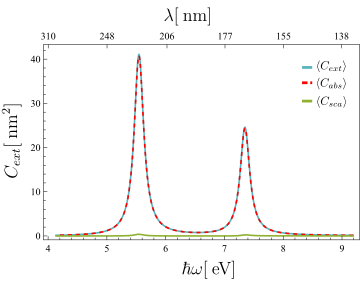
\includegraphics[width=.445\textwidth]{../../Figuras/AlContribuciones3.pdf} \label{Contribuciones}}\quad%
	\sidesubfloat[]{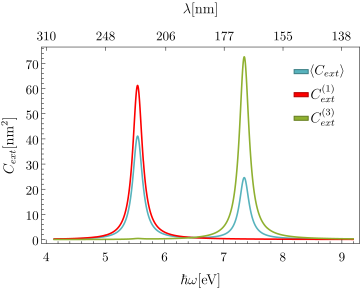
\includegraphics[width=.44\textwidth]{../../Figuras/CextAlbueno.pdf}\label{Cextpromedio}}%
	\caption{Secciones transversales como función de la energía $\hbar\omega$ (eje inferior) y de la longitud de onda $\lambda$ (eje superior) para una partícula elipsoidal oblata de aluminio caracterizada por su función dieléctrica dada por el modelo de Drude ($\hbar\omega_p=13.142\text{ eV}$, $\hbar\gamma=0.197\text{ eV}$), con semiejes $a=b=1.5\text{ nm}$, $c=1\text{ nm}$ e inmersa en un medio acuoso ($\epsilon_m=1.77$). \textbf{a)}~Sección transversal de absorción promedio $\langle C_{ext}\rangle$  del elipsoide (línea verde oscuro) y la esfera (línea roja punteada) y sección transversal de esparcimiento promedio $\langle C_{abs}\rangle$  del elipsoide (línea verde claro) y la esfera (línea naranja punteada) en escala logarítmica. \textbf{b)} Sección transversal de extinción promedio $\langle C_{ext}\rangle$ (línea azul), sección transversal de extinción al iluminar a la partícula con una onda polarizada en la dirección $\hat{e}_x$, $C_{ext}^{(1)}$  (línea roja)  y sección transversal de extinción al iluminar la partícula con una onda polarizada en la dirección $\hat{e}_z$ $C_{ext}^{(3)}$  (línea verde).} \label{fig:test}
\end{figure}

A partir de los resultados mostrados en la Fig. \ref{Contribuciones}, se observa que, en partículas dentro del régimen cuasiestático, la absorción domina sobre el esparcimiento en la contribución a la extinción. Esto se evidencia en la diferencia de magnitudes las curvas de absorción y esparcimiento de la esfera y la elipse, donde la absorción es aproximadamente tres órdenes de magnitud mayor que el esparcimiento, por lo que la curva de extinción es escencialmente la misma que la de absorción. Debido a esta marcada diferencia, los análisis posteriores se enfocan exclusivamente en las secciones transversales de extinción, ya que la contribución del esparcimiento es despreciable.\\

El análisis de las diferencias entre la $\langle C_{ext}\rangle$ y  las secciones transversales de extinción obtenidas al iluminar la partícula con una onda polarizada en una única dirección, se presenta en la Fig. \ref{Cextpromedio}. En esta figura se muestra la $\langle C_{ext}\rangle$ (línea azul), $C_{ext}^{(1)}$ (línea roja) y $C_{ext}^{(3)}$ (línea verde) de un elipsoide y la $\langle C_{ext}\rangle$ (línea gris punteada) de una esfera. Las cantidades se muestran en función de $\hbar\omega$ (eje inferior) y de $\lambda$ (eje superior) de la onda electromagnética incidente. Estos cálculos corresponden a un sistema con las mismas características que el de la Fig. \ref{Contribuciones}. Se observa que debido a la geometría, la 
$\langle C_{ext}\rangle$ del elipsoide presenta dos máximos, los cuales coinciden con las frecuencias de los máximos de $C_{ext}^{(1)}$ y $C_{ext}^{(3)}$ que se encuentran hacia el rojo y al azul, respectivamente, de la frecuencia de resonancia correspondiente a una partícula esférica. Esto muestra que las secciones transversales promedio son útiles para representar el efecto de iluminar una partícula elipsoidal con una onda electromagnética polarizada en la dirección de cualquiera de sus tres ejes principales, ya que lo que cambia es el valor nominal de los máximos en la sección transversal promedio, más no la localización espectral de estos. \\

Las siguientes figuras presentan los cálculos de las secciones tranversales de extinción promedio  $\langle C_{ext}\rangle$ considerando nanopartículas elipsoidales oblatas cuya función dieléctrica está caracterizada por el modelo de Drude para aluminio \cite{Aluminio} y por datos experimentales para plata \cite{Plata}, oro \cite{Plata}, bismuto \cite{Bismuto} y  óxido de magnesio \cite{MgO}.


\subsection*{Aluminio y plata}
En la Fig. \ref{aluminioplataAR} se muestran las $\langle C_{ext}\rangle$ en función de $\hbar\omega$ (eje inferior) y de  $\lambda$ (eje superior) de la onda electromagnética incidente en nanopartículas elipsoidales oblatas de aluminio (AlNPs) [Fig. \ref{aluminioAR}] y plata (AgNPs) [Fig.~\ref{plataAR}]. La función dieléctrica para el aluminio está dada por el modelo de Drude con parámetros $\hbar\omega_p=13.142\text{ eV}$, $\hbar\gamma=0.197\text{ eV}$, mientras que para la plata  está dada a partir de los datos experimentales reportados pr Johnson y Christy \cite{Plata}. Se realizan los cálculos para partículas elipsoidales con razón de aspecto AR=2 y con semiejes de tamaños desde 1 nm a 2.5 nm, en pasos de 0.5 nm; cada caso se identifica con el código de color mostrado en la gráfica. Además, se incluyen los cálculos para una partícula esférica con $a=2 \text{ nm}$ (línea gris punteada) y con razón de aspecto AR$=1$. Todas las partículas están  inmersas en un medio acuoso con $\epsilon_m=1.77$.\\

\begin{figure}[h!]
	\sidesubfloat[]{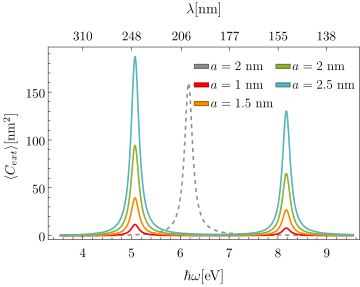
\includegraphics[width=.445\textwidth]{../../Figuras/AlAR} \label{aluminioAR}}\quad%
	\sidesubfloat[]{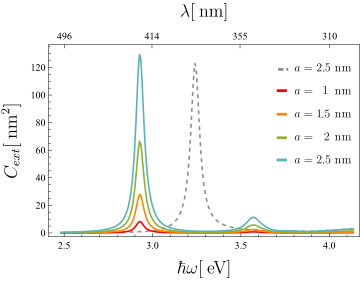
\includegraphics[width=.44\textwidth]{../../Figuras/AgAR}\label{plataAR}}%
	\caption{Secciones transversales de extinción promedio como función de la energía (eje inferior) y de la longitud de onda (eje superior) de la onda electromagnética incidente para una partícula elipsoidal oblata inmersa en un medio acuoso ($\epsilon_m=1.77$). Las partículas poseen AR=2, excepto en el caso de la línea gris punteada en el que AR=1 (partícula esférica). Además, están caracterizadas por su función dieléctrica dada por  \textbf{a)} el modelo de Drude para el aluminio con parámetros $\hbar\omega_p=13.142\text{ eV}$ y $\hbar\gamma=0.197\text{ eV}$) y \textbf{b)} datos experimentales correspondientes a la plata obtenidos de \cite{Plata}. }\label{aluminioplataAR}
\end{figure}
A partir de los resultados de la Fig. \ref{aluminioplataAR}, se observa que al aumentar el tamaño de la partícula mientras se mantiene constante AR, la localización espectral de las resonancias no cambia pero su valor nominal aumenta. Se identifican dos máximos locales en $\langle C_{ext}\rangle$,  los cuales corresponden a las frecuencias en las que $C_{ext}^{(1)}$ y $C_{ext}^{(3)}$ se maximizan. En ambos casos se observa que el corrimiento  de la resonancia no es simétrico respecto al de la esfera, para $C_{ext}^{(1)}$, las resonancias presentan un corrimiento hacia el rojo de $\Delta\lambda=$44 nm (1.11 eV) para las AlNPs y $\Delta\lambda=$51 nm (0.38 eV) para las AgNPs. Para $C_{ext}^{(3)}$, las resonancias presentan un corrimiento hacia el azul de $\Delta\lambda=$55 nm (2.33 eV) para AlNPs y $\Delta\lambda=$39 nm (0.36 eV) para las AgNPs. Es decir, este corrimiento depende del material.\\

El efecto de la variación de la razón de aspecto en la sección transversal de extinción promedio en AlNPs y AgNPs inmersas en un medio acuoso con $\epsilon_m=1.77$ se muestra en la Fig. \ref{aluminioplatac}. En esta figura, las partículas elipsoidales se consideran con AR entre 1.5 a 2.25, con incrementos 0.25 y con un semieje menor fijo de $c=1\text{ nm}$ y también se incluye $\langle C_{ext}\rangle$ para una partícula esférica con  $c=1\text{ nm}$ y con razón de aspecto AR$=1$.


\begin{figure}[h!]
	\sidesubfloat[]{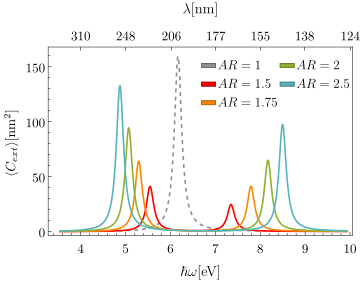
\includegraphics[width=.445\textwidth]{../../Figuras/Alc} \label{aluminioc}}\quad%
	\sidesubfloat[]{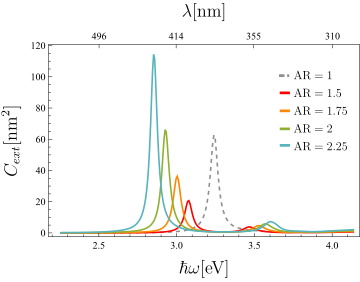
\includegraphics[width=.44\textwidth]{../../Figuras/Agc}\label{platac}}%
	\caption{Secciones transversales de extinción promedio como función de la energía (eje inferior) y de la longitud de onda (eje superior) de la onda electromagnética incidente para una partícula elipsoidal oblata inmersa en un medio acuoso ($\epsilon_m=1.77$). Las partículas  poseen un semieje menor de tamaño $c=1nm$ y presentan diferentes AR cuyo código de color se observa en la gráfica. Además, están inmersas en un medio acuoso ($\epsilon_m=1.77$) y están caracterizadas por su función dieléctrica dada por  \textbf{a)} el modelo de Drude para el aluminio ($\hbar\omega_p=13.142\text{ eV}$, $\hbar\gamma=0.197\text{ eV}$) y \textbf{b)} datos experimentales correspondientes a la plata obtenidos de \cite{Plata}.}\label{aluminioplatac}
\end{figure} 

 En las Figs. \ref{aluminioc}  y \ref{platac} se observa que conforme la relación de aspecto se aproxima a la unidad, hay un corrimiento de las frecuencias asociadas a las $\langle C_{ext}\rangle$ máximas hacia la frecuencia de resonancia asociada a una partícula esférica. Esta frecuencia de resonancia corresponde a $\lambda=201\text{ nm}$ (6.17 eV) para el aluminio y $\lambda=383\text{ nm}$ (3.24 eV) para la plata. Además, tanto en el aluminio como en la plata, se observa que al aumentar la relación de aspecto y la longitud del eje mayor, el valor nominal de  $\langle C_{ext}\rangle$ también aumenta. Esto se debe a que hay una mayor cantidad de material y por tanto más electrones, por lo que los efectos de absorción y esparcimiento aumentan, lo que, en consecuencia, aumenta la extinción.



\subsection*{Oro y bismuto}
De forma análoga al análisis en la variación de los parámetros geométricos de las AlNPs y AgNPs, se muestra en la Fig. \ref{oro} la respuesta óptica variando estos parámetros (semieje mayor y razón de aspecto) considerando ahora una función dieléctrica de materiales reales donde se observan contribuciones no descritas por el modelo de Drude. \footnote{Estas contribuciones provienen de electrones ligados \cite{Plasmonics}.} En particular, en la Fig. \ref{oroAR} se grafica $\langle C_{ext}\rangle$ como función de $\hbar\omega$ (eje inferior) y de $\lambda$ (eje superior) para nanopartículas elipsoidales oblatas de oro (AuNPs) de distintos tamaños que conservan la razón de aspecto de AR=2. Para complementar el análisis, se muestra debajo de esta gráfica la función dieléctrica del oro donde los puntos representan datos experimentales \cite{Plata} y las líneas continuas corresponden a la interpolación empleada para este conjunto de datos. En la Fig. \ref{oroAR} se consideran partículas con relación de aspecto AR$=2$ con radios desde 1  nm a 2.5 nm, con incrementos de 0.5 nm; cada caso se identifica con el código de color mostrado en la gráfica respectiva. También se considera una partícula con relación de aspecto AR$=1$ y semiejes $a=2$ nm (línea gris punteada), que representa a una partícula esférica. Por otro lado, en la Fig. \ref{oroc} se consideraron partículas con relación de aspecto variable AR=1.5 (línea roja), AR=1.75 (línea naranja), AR=2 (línea verde) y AR=2.25 (línea azul) que presentan valores en su semieje menor $c=1\text{ nm}$. Asimismo, se considera una partícula esférica con semieje mejor $c=1\text{ nm}$ y con relación de aspecto AR$=1$ (línea gris).
\begin{figure}[H]
	\sidesubfloat[]{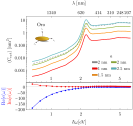
\includegraphics[width=.445\textwidth]{../../Figuras/Au2.pdf} \label{oroAR}}\quad%
	\sidesubfloat[]{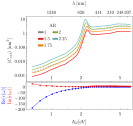
\includegraphics[width=.44\textwidth]{../../Figuras/Au.pdf}\label{oroc}}%
	\caption{Secciones transversales de extinción promedio como función de la energía (eje inferior) y de la longitud de onda (eje superior) para una partícula elipsoidal oblata de oro inmersa en un medio acuoso con $\epsilon_m=1.77$, y cuyo índice de refracción complejo fue obtenido a partir de datos experimentales de \cite{Plata}. Debajo de las gráficas se muestra la función dieléctrica del oro obtenida a partir de \cite{Plata} (parte real en azul, parte imaginaria en rojo). La línea recta que une los puntos experimentales fue obtenida mediante una interpolación. \textbf{a)} AuNPs con AR=2, excepto en el caso de una esfera (línea gris punteada) donde AR=1. \textbf{b)} AuNPs con semieje menor $c=1$ nm.}\label{oro}
\end{figure}

En contraste con el aluminio y la plata, para el oro se observa solo una excitación plasmónica en $\lambda=$ 522 nm (2.38 eV). Esta excitación presenta un corrimiento hacia el rojo de la de la esfera en $\lambda=$ 547 nm (2.27 eV) y se esperaría que existiera otra con un corrimiento hacia el azul, más no hay una excitación a frecuencias mayores como sí se observó en el análisis de la Fig. \ref{aluminioplataAR}. Esto se atribuye a la fuerte absorción del oro a energías altas, lo que suprime resonancias atribuidas a contribuciones no descritas por el modelos de Drude en los datos experimentales.\footnote{En particular de contribuciones dieléctricas descritas por el modelo de Lorentz \cite{Plasmonics}.} Por otro lado, se observa que para AR=2.25, la excitación se encuentra en $\lambda=$ 556 nm (2.23~eV), mientras que para AR=1.5, el caso calculado más cercano al de una esfera, la excitación se encuentra en $\lambda=$~522~nm (2.33~eV), es decir, la AR reproduce el caso de una esfera en su respuesta espectral cuando tiende a la unidad, resultado que sigue las tendencias observadas en las AlNPs y AgNPs.\\

En los casos anteriores se analizó el aluminio, cuya respuesta óptica es bien descrita por el modelo de Drude, así como metales nobles como la plata y el oro. Ahora, con el objetivo de aproximarse a las propiedades ópticas de los eritrocitos, en la Fig. \ref{bismuto} se presentan las secciones transversales de extinción promedio en función de la energía (eje inferior) y la longitud de onda (eje superior) para nanopartículas elipsoidales oblatas de bismuto (BiNPs). Este material, al ser un semimetal, exhibe en ciertas regiones espectrales un comportamiento más similar al de los eritrocitos que los materiales previamente estudiados. Como complemento, debajo de las gráficas se muestra la función dieléctrica del bismuto obtenida de datos experimentales reportados por Hagemann et al. \cite{Bismuto}. En la Fig. \ref{bismutoAR} se consideraron partículas con  AR$=2$  y en la Fig. \ref{bismutoc} se consideraron partículas con relación de aspecto variable desde 1.5 hasta 2.25, con incrementos de 0.25. 

\begin{figure}[H]
	\sidesubfloat[]{\includegraphics[width=.445\textwidth]{../../Figuras/Bi2} \label{bismutoAR}}\quad%
	\sidesubfloat[]{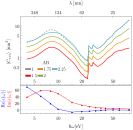
\includegraphics[width=.44\textwidth]{../../Figuras/Bi}\label{bismutoc}}%
	\caption{Secciones transversales de extinción promedio  como función de la energía (eje inferior) y de la longitud de onda (eje superior) para una partícula elipsoidal oblata de bismuto inmersa en un medio acuoso con $\epsilon_m=1.77$, y cuyo índice de refracción complejo fue obtenido a partir de datos experimentales de \cite{Bismuto}. Debajo de las gráficas se muestra la función dieléctrica del oro obtenida a partir de \cite{Plata} (parte real en azul, parte imaginaria en rojo). La línea recta que une los puntos experimentales fue obtenida mediante una interpolación. \textbf{a)} BiNPs con AR=2, excepto en el caso de una esfera (línea gris punteada) donde AR=1. \textbf{b)} BiNPs con semieje menor $c=1$ nm.}\label{bismuto}
\end{figure}

En ambas figuras se observan frecuencias de resonancia alrededor de $\lambda=147$ nm (8.44 eV), que se encuentran hacia el azul de la frecuencia de resonancia en $\lambda=154$ nm (8.03 eV) correspondiente a una nanopartícula esférica y de manera similar al caso del oro, se esperaría que existiera otra resonancia hacia el rojo de la de la esfera. También se observa un aumento de la $\langle C_{ext}\rangle$ a partir de $\lambda=50$ nm  que se atribuye a contribuciones no descritas por el modelo de Drude en los datos experimentales. Como en los casos anteriores, se observa que al aproximar AR a la unidad, se recupera la frecuencia de resonancia correspondiente a una nanopartícula esférica. Además, las excitaciones plasmónicas están menos definidas que en el caso de los materiales plasmónicos. Esto es más evidente al comparar la Anchura a media altura (FWHM por sus siglas en inglés) pues, en el caso del bismuto se observa un FWHM = 8.85 nm (0.18 eV), mientras que en el aluminio FHWM = 68.54 nm (3.64 eV). Esto se explica debido a la fuerte absorción del bismuto en el rango de frecuencias estudiado.





\subsection*{Óxido de magnesio}
Finalmente, las $\langle C_{ext}\rangle$ para un material dieléctrico: el óxido de magnesio (MgO) se muestran en la Fig. \ref{mgo}, en las que se emplearon los datos experimentales reportados por Stephens y Malitson \cite{MgO}. En esta gráfica se realiza la variación de la AR y el semieje mayor en nanopartículas elipsoidales oblatas de óxido de magnesio (MgONPs). Las $\langle C_{ext}\rangle$ se grafican en función de la energía (eje inferior) y de la longitud de onda (eje superior). De la misma forma que con los materiales anteriores, se consideraron partículas con relación de aspecto AR$=2$ con radios desde 1  nm a 2.5 nm, con incrementos de 0.5 nm, con su respectivo código de color indicado en la gráfica [Fig. \ref{mgoAR}] y en la Fig. \ref{mgoc} se consideraron partículas con AR variable. 

\begin{figure}[H]
	\sidesubfloat[]{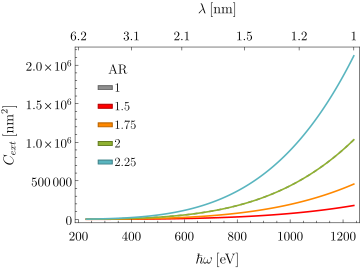
\includegraphics[width=.445\textwidth]{../../Figuras/MgOc} \label{mgoc}}\quad%
	\sidesubfloat[]{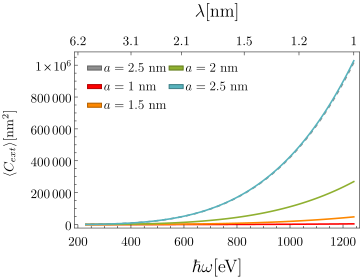
\includegraphics[width=.44\textwidth]{../../Figuras/MgOAR}\label{mgoAR}}%
	\caption{Secciones transversales de extinción promedio como función de la energía (eje inferior) y de la longitud de onda (eje superior) para una partícula elipsoidal oblata de óxido de magnesio inmersa en un medio acuoso ($\epsilon_m=1.77$). \textbf{a)} MgONPs con AR=2, excepto en el caso de una esfera (línea gris punteada) donde AR=1. \textbf{b)}  MgONPs con semieje menor $c=1$ nm.}\label{mgo}
\end{figure}

En ambos casos se observa que la $\langle C_{ext}\rangle$ tiene un comportamiento creciente y no se observan resonancias plasmónicas debido a la naturaleza dieléctrica del óxido de magnesio. Esto también se atribuye a que en el rango de energías analizado existen procesos de absorción no descritos por el modelo de Drude.









\section{Conclusiones}
La respuesta óptica de elipsoides de distintos materiales y tamaños dentro de la nanoescala se caracterizó a través del cálculo de las secciones transversales de absorción, esparcimiento y extinción, bajo la aproximación cuasiestática, para nanopartículas elipsoidales oblatas de aluminio, plata, oro, bismuto y óxido de magnesio. Se encontró que, en el límite cuasiestático, la absorción es la contribución predominante en la extinción, mientras que el esparcimiento resulta despreciable. En el rango donde los materiales presentan un comportamiento acorde con el modelo de Drude, se identificaron dos resonancias plasmónicas correspondientes a la iluminación de los elipsoides en las direcciones $\hat{e}_x$ y $\hat{e}_z$, ubicadas hacia el rojo y el azul, respectivamente, de la frecuencia resonancia observada para una nanopartícula esférica. Por otro lado, en los rangos en los que la función dieléctrica de los materiales no se ajusta al modelo de Drude, el incremento en la sección transversal de extinción promedio se asocia con contribuciones descritas por el modelo de Lorentz. Finalmente, para las partículas de óxido de magnesio, se observó que la sección transversal de extinción aumenta con la energía, lo que se atribuye a su naturaleza dieléctrica.


\bibliographystyle{ieeetr}
\bibliography{Referencias}


%----------------------------------------------------------------------------------------
\end{document}
